\documentclass{../template/texnote}

\title{\textbf{\capitalisewords{A sneak peak into the science behind telescopes}}}

\begin{document}
    \maketitle \currentdoc{note}
    %<*note>

To the untrained human eye, most objects in the night sky resemble stars. However, to the astronomer they become planets, galaxies, nebulae, Active Galactic Nuclei (AGNs), supernovae or even the International Space Station (ISS).
When Galileo Galilei used the telescope to look into the heavens for the first time, a whole new world slid into view. That historical moment was part of a sequence of events that would usher in the scientific revolution and subsequently change mankind's history.
%Astronomy is often said to be the precursor of all  sciences.
%Although the first telescopes were invented in 16th century Netherlands by spectacle makers Hans Lippershey \& Zacharias Janssen, Galileo Galilei was one of the first people to use them to view the heavens.
Today's astronomical surveys employ the latest and greatest in terms of telescopes and imaging systems. These large telescope systems do not have individual astronomers sitting behind them to view the sky. Rather images of the sky are continuously taken and stored in large data centers for further processing and analysis.
%Astrophotography is the term given for imaging astronomical objects or regions of the night sky.
% How does the telescope benefit the astronomer? Is it by increasing the farthest distance upto which he can see or making objects appear magnified?
%Contrary to popular conception, telescopes enables astronomers to see faint objects and not distant objects. The human eye by itself is a wondrous device that enables us to see objects as distant as 2.5 million light years (the Andromeda Galaxy).
%To understand astrophotography, you need an understanding of the basics of photography. Knowing some of these ideas will also help you to understand the design and workings of telescopes which we will explore in a future article. In this article, we will get acquainted with basic terminologies in photography and the physics behind them.
%How do telescopes enable the observer to see beyond the capacities of their own eyes?
%There is a lot of interesting science behind the working of telescopes.
Take the homepage of any astronomical survey and you are bound to find terms like the aperture size, field of view and the number of megapixels among the specifications. Let us try to understand the  relevance of these parameters in observational astronomy and the science behind them with the help of the humble pinhole camera.
\section{Importance of Aperture}
Contrary to popular perception, the utility of a telescope is not in its ability to make distant objects visible. The human eye by itself is capable of viewing upto a distance of 2.5 million light years (the Andromeda Galaxy). Telescopes are beneficial to the astronomer because of two things, they make faint objects appear brighter (light gathering power) and they allow objects that are seen as a single entity to be separated into its parts (resolving power).
Both these depend to a large extent on the aperture size of the telescope objective.
\begin{figure}
\begin{tabular}{cc}
  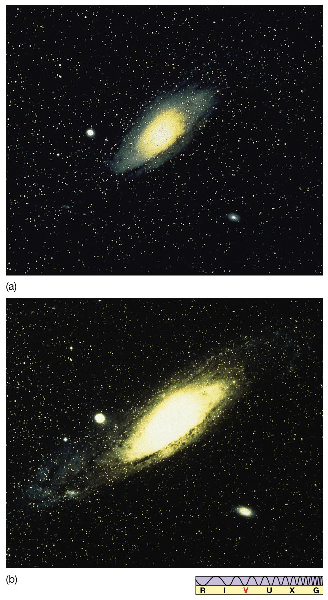
\includegraphics[width=70mm]{Linn/light-gathering.png} &   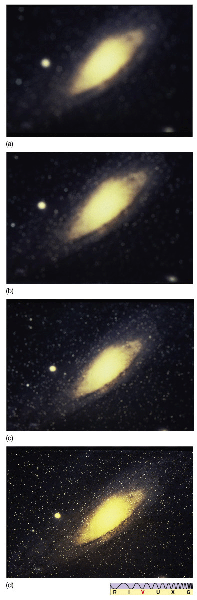
\includegraphics[width=42 mm]{Linn/resolving.png} \\
%(a) first & (b) second \\[6pt]
\end{tabular}
\caption{On the left, Two images showing the effect of lesser (top) and greater (bottom) light gathering power.
On the right,
Images showing the effect of worse (top) to better (bottom) resolving power. (Image Courtesy: Chaisson/McMillan, Astronomy-4th edition))
}
\label{fig:pinhole_cam}
\end{figure}

% \section*{Revisiting the pinhole camera}
What is the importance of aperture in a telescope?
Let's start that discussion by first defining what an image is. In the most elementary terms, an image is the representation of a physical object. So by definition, an image is not a real object; it's unreal. But images themselves are classified as ``real" or ``virtual."
A ``real image" is where real light rays join together; hence, they can be caught on a screen. A virtual image like the one you see in a plane mirror appears to come from some point behind the mirror - yet if you go behind the mirror, you cannot find it.
Let's limit our discussion to real images for now.
All you need to get a ``real" image of something, is a pinhole camera. Let's revisit the pinhole camera experiment that we were introduced to, in
%maybe familiar with starting from
elementary school. The basic setup needed to make a pinhole camera is pretty simple. Take an empty cardboard box with one side open. Cover the open side using a translucent paper; this becomes the screen. On the opposite side of the screen, make a hole using a pin. Keep this setup in a darkened room with only a candle flame as the light source.  After adjusting the distance of the candle from the pinhole, voila!, an inverted image appears on the screen.

\begin{figure}
    \centering
    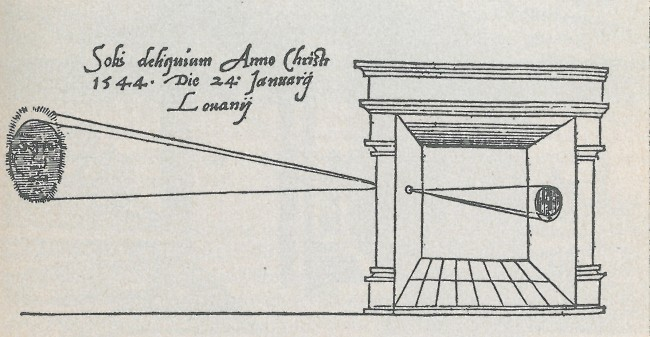
\includegraphics[scale=.5]{Linn/camera-obscura.jpg}
    \caption{\textbf{Camera Obscura}. The earliest published drawing of a camera obscura can be found in Gemma Frisius' 1545 book De Radio Astronomica et Geometrica. In the book, Frisius, a Dutch physician, mathematician, and instrument maker, describes and shows how he used the camera obscura to observe the solar eclipse of 24 January 1544. (Image Courtesy: Wikipedia.org)}
    \label{fig:my_label}
\end{figure}

%\section*{Why do images appear blurred?}
%\section*{How does a pinhole camera work? }
% \section*{Apertures versus Lenses}
Why did we need an aperture in the first place? What prevents an image from forming, in absence of a pinhole ?
The pinhole acts like a filter allowing only light rays that come from a particular point on the object and in a particular direction to reach the screen.
If you increase the size of the aperture, each point on the screen starts to receive light rays from different parts of the scene. And if the aperture becomes sufficiently large the image gets completely washed out.
This is illustrated in Figure \ref{fig:pinhole_cam}.
\begin{figure}
\begin{tabular}{cc}
  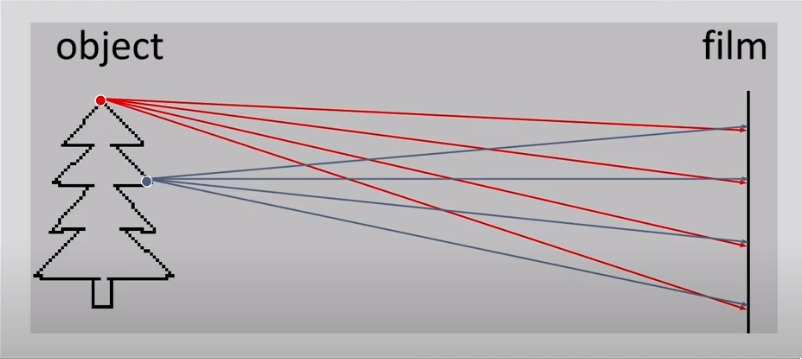
\includegraphics[width=70mm]{Linn/pc1.png} &   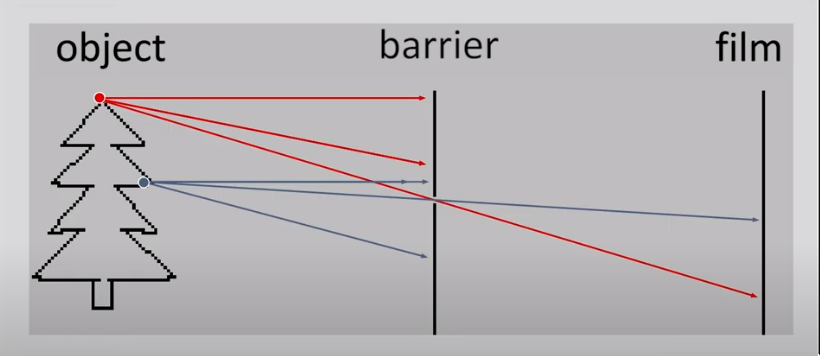
\includegraphics[width=72mm]{Linn/pc2.png} \\
%(a) first & (b) second \\[6pt]
\end{tabular}
\caption{Without a barrier, there will be no image as all points on the screen receive light rays from multiple points on the scene. (Image Courtesy: Udacity)
}
\label{fig:pinhole_cam}
\end{figure}
%\section*{The role of lenses }
But, if a pinhole is sufficient to create an image, why do you need a lens? We saw that with pinholes, in order to get a sharp image, you need to have a sufficiently small aperture. This has the undesired effect of making the image dim. A pinhole cuts out a lot of parallel rays coming from adjacent points on the object.
A convex lens solves this issue as it can bend parallel rays onto a single point.
Even though lenses replace the aperture in a pinhole camera, modern camera lenses do have an aperture added on top of the lens similar to a pinhole.
In such a case, the aperture size of the lens refers to the actual diameter of the lens itself.
Thus lenses help us to collect light coming from a very large area much larger than the size of our pupil and focuses them onto a point making even faint objects visible.

% \section*{Focus and the Point Spread Function}


% Consider an object placed in front of a pinhole camera. Each point on the screen receives light coming from a single point on the object and in a single direction. However, with a convex lens, rays of light that start out from a single point on the object and traveling along different directions converge to the corresponding image point. When this happens for all the points on the object, we say that the image is focused.

% For objects that are far away from the lens, the screen can be placed at the principal focus to get a focused image. Now, if the object is brought closer, the image appears to get blurrier or go out of focus. This is because the plane where all the points of convergences lie has moved either behind or in front of the screen. On the screen, however, each point on the object has spread out, forming a circle. This is called the point spread. The screen needs to be adjusted in order to bring the object back into focus.

% \section*{Controlling the aperture for taking better photos}
% Have you ever wondered how modern DSLR cameras can be used to take stunning photos with the so called 'Bokeh' effect? And why such effects are not easily reproduced with your average smartphone camera?
% The reason is that the aperture in a DSLR camera enables you to control something called the depth of field.
% % \section*{What  is the depth of field?  }
% % \begin{figure}
% %     \centering
% %     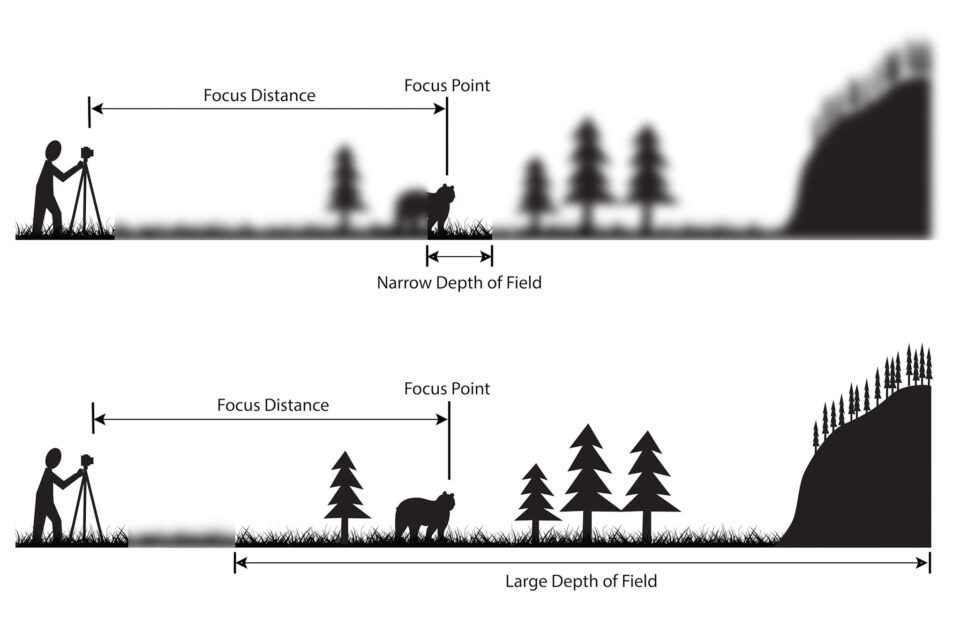
\includegraphics[scale=0.5]{DoF-sketch-960x624.jpg}
% %     \caption{Depth of field.}
% %     \scriptsize{Image Credit : https://photographylife.com/what-is-depth-of-field}
% %     \label{fig:my_label}
% % \end{figure}
% Consider an object that has been sharply focused on our screen. What happens if we make a slight adjustment to the screen? Does the image go entirely out of focus? Probably not. There is a range where the rays are close enough to be considered sharp. This is called the depth of field. Or, equivalently, the depth of field is said to be the distance through which the subject can move without the image going entirely out of focus. Note that the aperture is not the only thing that affects the depth of field, the focal length of the lens also does.

% With pinholes, the aperture size is related to the focal length, which is how far you want the image to be focused.
%Even though lenses are used as a replacement for pinholes, they still use an aperture. In modern cameras, the depth of field is controlled by lens and aperture.


% \begin{figure}
%     \centering
%     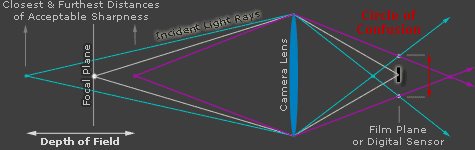
\includegraphics{dof_lensdiagram.png}
%     \caption{Ray diagram showing the depth of field and the circle of confusion}
%     \label{fig:my_label}
%     Image credit: https://www.cambridgeincolour.com/tutorials/depth-of-field.htm
% \end{figure}

% \begin{figure}
%     \centering
%     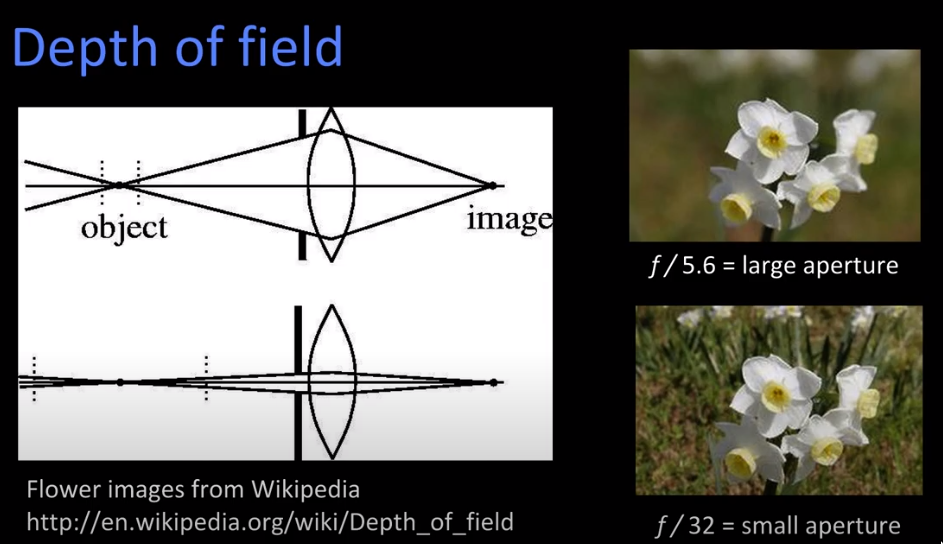
\includegraphics[scale=0.5]{DoF2.png}
%     \caption{The effect of aperture on the depth of field}
%     \label{fig:my_label}
% %    Image credit: https://www.cambridgeincolour.com/tutorials/depth-of-field.htm
% \end{figure}

% \section*{Apertures and the exposure triangle}

% Using an aperture has other interesting consequences. Increasing the aperture lets you capture more light within a dimly lit scene. This also lets you compensate for faster shutter speeds when capturing moving objects. Similarly, slower shutter speeds compensate for smaller apertures by letting in more light onto the sensor. The third element in this triangle is the ISO, a setting used to artificially make the image brighter by increasing the sensitivity of pixels to light (or the amplification of the light received). Increasing the ISO has the downside of introducing more noise into your image. Thus these three things need to be considered together, forming what is called the exposure triangle.

% \section*{ What is the relation between focal length and field of view? }
%\section*{Why do your selfies look weird?}

% \section*{Image magnification}
% \section*{The difference between digital zoom and optical zoom}
\section{Focal length, Field of View and Image magnification}
Returning to the pinhole camera, let's see what happens when you increase the distance between the hole and the screen. In the image that is formed, subjects close to the camera grow in size, whereas parts of the background are lost.
When this happens, we say that the field of view decreases. In the case of a pinhole camera, the distance between the hole and the screen is called the focal length. Thus the field of view decreases when the focal length increases and conversely, when the focal length decreases, the field of view increases. This is seen in the animation shown in Figure \ref{fig:pinhole_focal}
Notice that the image that appears magnified
also appears dull and fuzzy. This is because the same information is now spread over a larger surface area.

This relation between the focal length and the field of view holds true even for lenses. This can be seen in figure \ref{fig:lens_focal}. The decreased field of view leads to higher magnification for lenses with a longer focal length. (Note that this is not the case with microsocopes where a shorter focal length leads to better magnification). Telescopes makes use of a compound lens system where the long focal length lens (objective) focuses an image of a distant object much closer to our eyes. This image can be much smaller than the actual object however it has a greater angular magnification as it is now much closer to our eyes. This image is now viewed through the eyepiece which further magnifies it. The total magnification of the telescope is the product of these two magnifications. Thus the magnification is not an essential feature of a telescope as it can be increased arbitrarily by increasing the magnification of the eyepiece.

However the resolving power of the telescope is a characteristic property which has a theoretical limit set by the equation $$\sin \theta \approx \theta = 1.22\lambda/D$$ Where D is the aperture of the telescope objective. Magnification beyond this limit is useless as no more resolution is obtained and the image ends up being mushy. The resolving power is further limited in modern digital cameras by the pixel size of the CCD sensors.
%$(Note: When your field of view is very narrow, it is best to mount the camera on a tripod, as even the slightest disturbance might cause an image blur. )


\begin{figure}
\begin{tabular}{cc}
  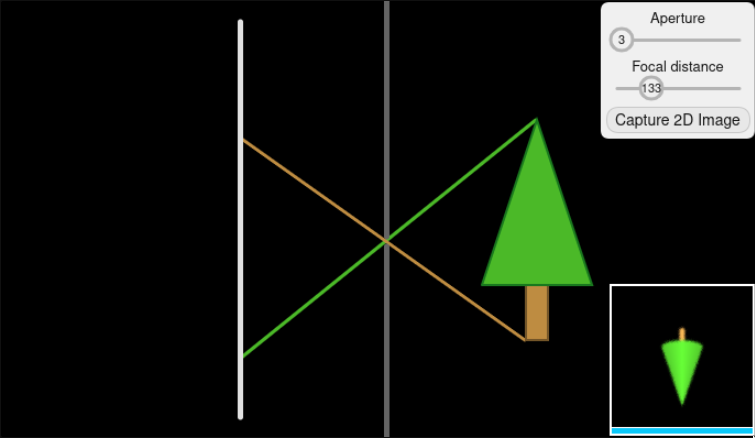
\includegraphics[width=75mm]{Linn/Pinhole_Focal.png} &   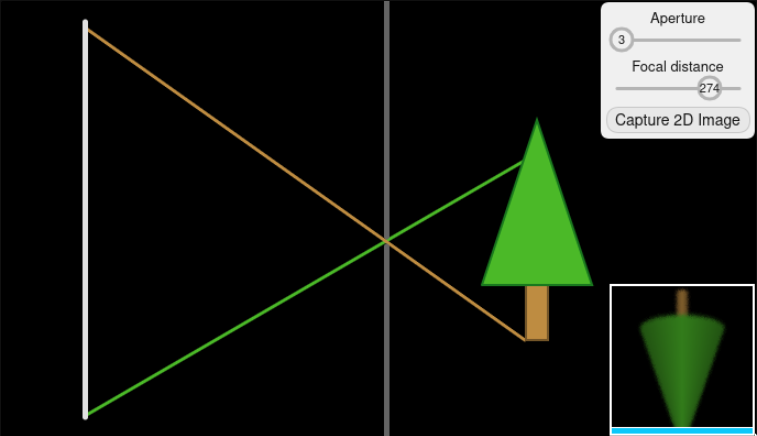
\includegraphics[width=75mm]{Linn/Pinhole_Focal2.png} \\
%(a) first & (b) second \\[6pt]
\end{tabular}
\caption{The effect of moving your screen away from the pinhole is a decreased field of view. The image
}
\label{fig:pinhole_focal}
\end{figure}



\begin{figure}
    \centering
    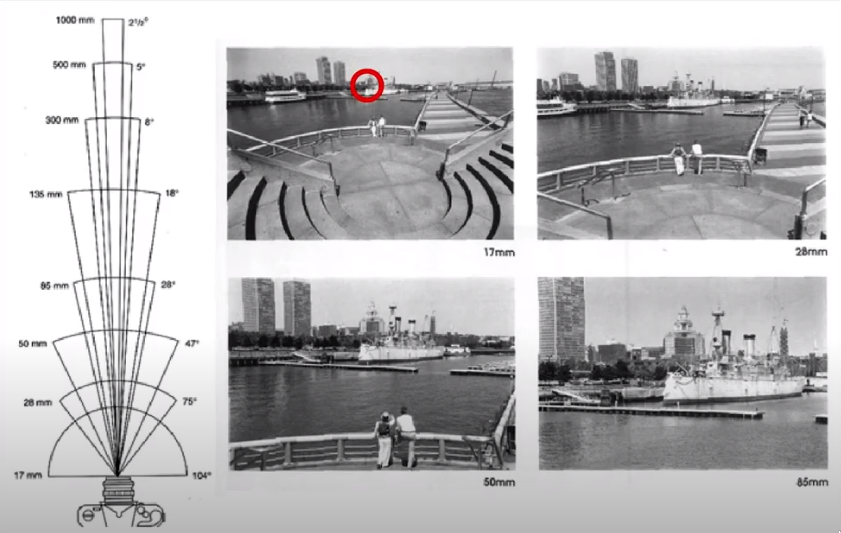
\includegraphics[scale=0.5]{Linn/FieldOfVIew.png}
    \caption{The larger the focal length of the lens used, the narrower the field of view. Image Courtesy: Udacity}
    \label{fig:lens_focal}
%    Image credit: https://www.cambridgeincolour.com/tutorials/depth-of-field.htm
\end{figure}

% \begin{figure}
%     \centering
%     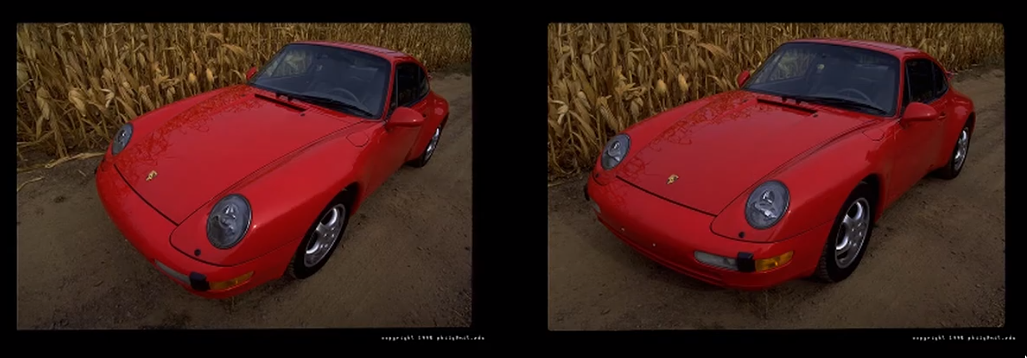
\includegraphics[scale=0.5]{FoV2.png}
%     \caption{The image on the left is taken using a lens with a larger field of view and hence the photographer had to move closer to the car to keep it at the same size as the other one. Image Courtesy: Udacity}
%     \label{fig:my_label}
% %    Image credit: https://www.cambridgeincolour.com/tutorials/depth-of-field.htm
% \end{figure}

%\section{ Relation between sensor size and field of view}

% \section*{What does it mean to have more megapixels? }



Finally, lets try to understand the importance of the number of megapixels that if often quoted with cameras. It can be seen from Figure \ref{fig:pinhole_focal} that because a longer focal length results in a wider field of view, the size of the screen needs to be sufficiently big in order to capture the entire scene.
With cameras, what this means is that when you talk about more megapixels (higher resolution) for a sensor, what you get is an increased field of view given the same optics, scene, and pixel size.
If you keep the sensor size the same and decrease the size of individual pixels, what you get is more digital zoom capability. Digital zoom lets you uncover details that otherwise would be washed out with a lower-resolution sensor. However this is often at the expense of reduced sharpness and increased noise in the image.
%However, if you really want to make use of the bigger field of view, you need to have a big enough screen. If you have a room with a very big window opposite a wall, you can use it as a pinhole camera with a very big screen and capture the image of a large area outside your room.

 %When you move toward the object, you do the opposite; you try to get more pixels on the target object (in the scene) at the cost of a reduced field of view. Note that moving in and zooming in is not the same thing.
%When you have more pixels on target, you can take a wide image capture of an object and then digitally zoom into the scene to uncover details that otherwise would be washed out or out of focus with a lower-resolution sensor.


% \medskip
% \textbf{Find-It-Out
% }
% Which is the largest camera used for astronomical surveys? Find out its sensor size and the field of view.

\section*{References}

\begin{enumerate}
    \item \url{    https://fpcv.cs.columbia.edu/}
\item \url{https://learn.udacity.com/courses/ud810}
\item \url{https://www.youtube.com/playlist?list=PL8dPuuaLjXtPAJr1ysd5yGIy}
\item \url{https://www.adimec.com/resolution-versus-field-of-view/}
\item \url{https://www.khanacademy.org/computing/pixar}
\end{enumerate}
    %</note>
    \printbibliography
\end{document}
